% !TeX root = ../libro.tex
% !TeX encoding = utf8



\setchapterpreamble[c][0.75\linewidth]{%
	\sffamily
  

    Las redes neuronales recurrentes son un tipo de redes neuronales un tanto más sofisticadas que las anteriormente vistas y muy usadas en la actualidad gracias a su capacidad para olvidar y recordar la información a través del tiempo. Se emplean principalmente para el procesamiento del lenguaje natural y en áreas en las que se trabajen con señales temporales, como es el caso del problema a tratar en la parte siguiente. \\
    
    El capítulo empezará con una introducción en la que detalla brevemente para qué se usan estas redes y qué posibilidades ofrecen frente a las redes neuronales prealimentadas. En la sección siguiente se dará una representación de las RNN usando grafos computacionales en donde la estructura recurrente queda visualmente más clara. Después se expondrá el funcionamiento de este tipo de redes comentando la variedad de diseños que se pueden realizar. Tras lo cual se detallará una generalización de este tipo de redes conocida como las redes recursivas que tienen una estructura de árbol profundo en lugar de una estructura de cadena. Para introducir los gruesos gordos del capítulo previamente se comentará un problema que afecta a las redes neuronales recurrentes, que es la dependencia a largo plazo, ocasionada por la explosión y/o desvanecimiento del gradiente. Dicho lo cual entran en juego los dos grandes tipos de redes neuronales recurrentes que solventan el problema anterior y que son las que se usarán en la práctica, LSTM (Long-Short Term Memory) y GRU (Gated Recurrent Unit). \\
    
    Las referencias empleadas para la elaboración de este capítulo ha sido principalmente el contenido del libro \textit{Deep Learning Book} \cite{Goodfellow-et-al-2016} y el material ofrecido por el contenido de un repositorio de \href{https://colah.github.io/posts/2015-08-Understanding-LSTMs/}{GitHub}
   

  
	\par\bigskip
}
\chapter{Redes Neuronales Recurrentes}\label{ch:RNN}

\newpage 
\section{Introducción}



        
        
        
    Las redes neuronales recurrentes o RNNs son un tipo de redes neuronales que procesan secuencias de datos, en concreto, procesan una secuencia de valores $x^{(1)},...,x^{(\tau)}$. Estas redes pueden manejar series mucho más largas que las redes neuronales convencionales. Para ir desde las redes multicapa a las recurrentes tenemos que aprovechar una de las primeras ideas del aprendizaje automático, compartir parámetros entre distintas partes del modelo. El hecho de compartir parámetros hace posible extender y poder aplicar el modelo a ejemplos de distinto tamaño y generalizar. Compartir parámetros es particularmente interesante cuando un trozo concreto de información puede aparecer en varias posiciones dentro de una secuencia. Por ejemplo, si consideramos dos frases \textit{Fui al Kilimanjaro en 2022} y \textit{En 2022, fui al Kilimanjaro}, nos gustaría que si le preguntásemos a un modelo de ML que leyera la frase y nos extrajera el año en el cual el narrador fue al Kilimanjaro, reconociera que fue en 2022. Si tuviéramos una red neuronal convencional, tendría parámetros separados para cada característica de entrada, por lo que necesitaría aprender todas las reglas de la lengua por separado en cada posición de la frase. \\
        
    Una idea parecida es el uso de convoluciones $1D$ para series temporales que permiten que una red poco profunda comparta parámetros a lo largo del tiempo. La salida de la convolución es una secuencia en la que cada miembro de la salida es una función en la que interviene un vecindario de la secuencia de entrada. Las RNN comparten parámetros de manera distinta. Cada miembro de la salida es una función de los miembros anteriores, y se producen usando la misma regla de actualización aplicada a las salidas anteriores. Esta formulación recurrente hace que se compartan los parámetros a través de grafo computacional. \\ 
        
    Para simplificar la notación, nos referimos a las RNNs como operaciones sobre una secuencia que contiene vectores $x^{(t)}$ con $t=1,...,\tau$ siendo t el paso de tiempo. En la prácticas las RNNs generalmente usan mini lotes de las secuencias con una longitud de secuencia diferente para cada miembro del mini lote. Pero hemos omitido los índices del mini lote para simplificar la notación. Otro detalle a tener en cuenta es que el índice del paso del tiempo no tiene por qué referirse literalmente al paso del tiempo en el mundo real, a veces también puede referirse a la posición en la secuencia. Las RNNs también pueden aplicarse en dos dimensiones, como en imágenes, e incluso a datos que implican tiempo. \\
        
    \section{Representación de RNN usando grafos computacionales}
        
    Los grafos computacionales nos permiten definir las RNNs. Recordemos que un grafo computacional es una manera de formalizar la estructura de un conjunto de cálculos. Para empezar, cada nodo de nuestro grafo será la representación de una variable de nuestro sistema, que pueden ser un escalar, vector, matriz, tensor o incluso una variable de otro tipo. Las conexiones o aristas de nuestro grafo representarán operaciones. Éstas pueden ser de una o varias variables del sistema (nodos) y deben ir a parar a otra de las variables. Distinguir entre las variables de entrada y las de salida lo haremos por la dirección que tenga la arista correspondiente. \\
    
    
    Vamos a explicar la idea de desplegar un cálculo recursivo o recurrente en un grafo computacional que tiene una estructura repetitiva, típicamente correspondiente a una cadena de eventos. Al desplegar el grafo, se comparten los parámetros en una estructura de red profunda. Por ejemplo, consideramos la forma clásica de un sistema dinámico
        
        \begin{equation}\label{eq:dinamy system}
                s^{(t)} = f(s^{(t-1)};\theta)
        \end{equation}
        
    \noindent donde $ s^{(t)}$ es el estado del sistema. Dicha ecuación \eqref{eq:dinamy system} es recurrente porque la definición de $s$ en un tiempo $t$ involucra al estado anterior. Fijando un periodo de tiempo finito $\tau$ podemos desplegar el grafo aplicando la definición $\tau - 1$ veces. Por ejemplo, para $\tau = 3$ tendríamos
        
        \begin{equation}
            \begin{aligned}
                s^{(3)} = f(s^{(2)}; \theta) = f(f(s^{(1)};\theta);\theta)
            \end{aligned}
        \end{equation}


    \noindent Entonces, si expandimos la ecuación todo lo que se pueda, llegaríamos al estado inicial del sistema y dicha expresión podría ser representada por un grafo computacional acíclico y dirigido.\\  
    
    
    Las redes neuronales recurrentes se pueden construir de varias maneras. Cualquier función que implique recurrencia puede considerarse una RNN. Muchas RNNs usan la ecuación \eqref{eq:rnn} o una parecida donde el estado $h$ representa una unidad oculta de la red y $x^{(t)}$ es una señal externa en el tiempo $t$.
        
            \begin{equation}\label{eq:rnn}
                h^{(t)} = f( h^{(t-1)} , x^{(t)} ; \theta)
            \end{equation}
            
    \noindent Generalmente, las arquitecturas RNNs incluyen capas adicionales como capas de salidas que leen la información del estado $h$ para hacer predicciones. \\
    
    
    
    \begin{figure}[H]
                \centering
                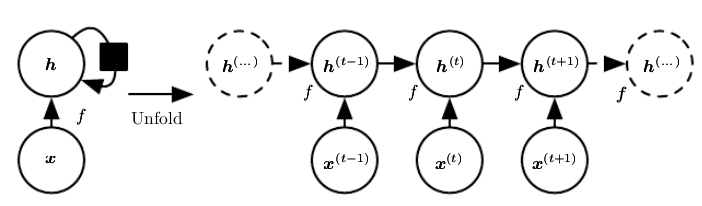
\includegraphics[height = 3cm, width = 10 cm]{img/grafo computacional 1.png}
                \caption{Una red recurrente sin salidas. Esta red solo procesa la información desde la entrada $x$ incorporándola al estado $h$ que se transmite hacia adelante a través del tiempo. (Izquierda) Diagrama del circuito, el cuadrado negro indica un retraso de un solo paso de tiempo. (Derecha) La misma red vista como un grafo desplegado, ahora cada nodo se asocia a una instancia temporal concreta. }
                \label{fig:grafo 1}
        \end{figure}
        
        
    Cuando se entrena a la red para realizar una predicción futura a partir del pasado, la red aprende a usar $h^{(t)}$ como una especia de resumen (con pérdidas) de los aspectos relevantes de la secuencia pasada de las entradas hasta el tiempo $t$. El resumen tiene pérdidas, ya que asigna una secuencia de longitud arbitraria, $x^{(t)},x^{(t-1)},...,x^{(2)},x^{(1)}$ a un vector de longitud fija $h^{(t)}$. Dependiendo del criterio de entrenamiento, este resumen podría conservar unos aspectos de la secuencia con más precisión que otros. \\
        
    La ecuación \ref{eq:rnn} puede dibujarse de dos maneras distintas. La primera es un diagrama que contiene un nodo para cada componente. Desde este punto de vista, la red define un circuito que funciona en tiempo real, con partes físicas cuyo estado actual puede influir en su estado futuro como en la izquierda de la figura \ref{fig:grafo 1}. El cuadrado negro se usa para indicar que la interacción tiene lugar con un retraso de un paso de tiempo, desde el estado en el tiempo $t$ al estado en el tiempo $t+1$. La segunda manera es desplegar el grafo, ahora cada componente está representada por muchas variables diferentes, con una variable por paso de tiempo que representa el estado de la componente en ese momento. Cada variable para cada paso de tiempo se dibuja como un nodo separado, como en la derecha de la figura \ref{fig:grafo 1}. \\ 
        
        
        
%%%%%%%%%%%%%%%%%%%%%%%%%%%%%%%%%%%%%%%%%%%%%%%%%%%%%%%%%%%%%%%%%%%%%%%%%%%%%%%%%%%%%
%%%%%%%%%%%%%%%%%%%%%%%%%%%%%%%%%%%%%%%%%%%%%%%%%%%%%%%%%%%%%%%%%%%%%%%%%%%%%%%%%%%%%
%%%%%%%%%%%%%%%%%%%%%%%%%%%%%%%%%%%%%%%%%%%%%%%%%%%%%%%%%%%%%%%%%%%%%%%%%%%%%%%%%%%%%


    \section{Funcionamiento de RNNs}
        
    La estructura y el proceso de despliegue de las RNNs introducen dos grandes ventajas: La primera es que independientemente de la longitud de la secuencia, el modelo aprendido siempre tiene el mismo tamaño de entrada porque la entrada se especifica en términos de la transición de un estado a otro en vez de estar especificada en términos una longitud variable de estados. La segunda es que es posible usar la misma función de transición $f$ con los mismos parámetros en cada paso de tiempo. Estos dos factores hacen posible el aprendizaje de un único modelo $f$ que opera en todos los pasos de tiempo y todas las longitudes de secuencia, en lugar de tener que aprender un modelo separado $g$ para todos los pasos de tiempo posibles. El aprendizaje de un único modelo compartido permite la generalización a longitudes de secuencia que no aparecen en el conjunto de entrenamiento y que permite que el modelo sea estimado con muchos menos ejemplos de entrenamiento de los que necesitaría en caso de que no se compartieran los parámetros. \\
        
    De acuerdo a lo anterior, se pueden diseñar una amplia variedad de RNNs. Algunos patrones de diseño importantes son los siguientes: 
        
            \begin{itemize}
                \item Redes recurrentes que producen una salida en cada paso de tiempo y tienen conexiones recurrentes entre las unidades ocultas. (Fig. \ref{grafo:rnn2})
                
                \item Redes recurrentes que producen una salida en cada paso de tiempo y tienen conexiones recurrentes sólo desde la salida en un paso de tiempo a las unidades ocultas en el siguiente paso de tiempo. (Fig. \ref{fig:rnn2tipo})
                
                \item Redes recurrentes con conexiones recurrentes entre las unidades ocultas que leen una secuencia completa y luego producen una única salida. (Fig. \ref{fig:rnn3tipo})
            \end{itemize}
            
        Vamos a explicar el funcionamiento de la RNNs de la figura \ref{grafo:rnn2} por ser bastante representativo. En dicha figura tenemos un grafo computacional que calcula la pérdida en el entrenamiento de una de una red recurrente que asigna una secuencia de entrada de valores $x$ a una secuencia de valores de salida $o$. Una pérdida $L$ mide lo lejos que está $o$ de la etiqueta del ejemplo de entrenamiento $y$. Cuando se usan las softmax como salidas suponemos que $o$ es un logaritmo de probabilidades y que no está normalizado. Entonces, $L$ internamente calcula $\hat{y} = softmax(o)$ y lo compara con $y$. La RNN tiene entradas a conexiones ocultas parametrizadas por una matriz de pesos $U$, conexiones recurrentes de unidades ocultas a unidades ocultas parametrizadas por una matriz de pesos $W$ y conexiones de unidades ocultas a salidas parametrizadas por una matriz de pesos $V$. \\
            
            
            \begin{figure}[ht]
                \centering
                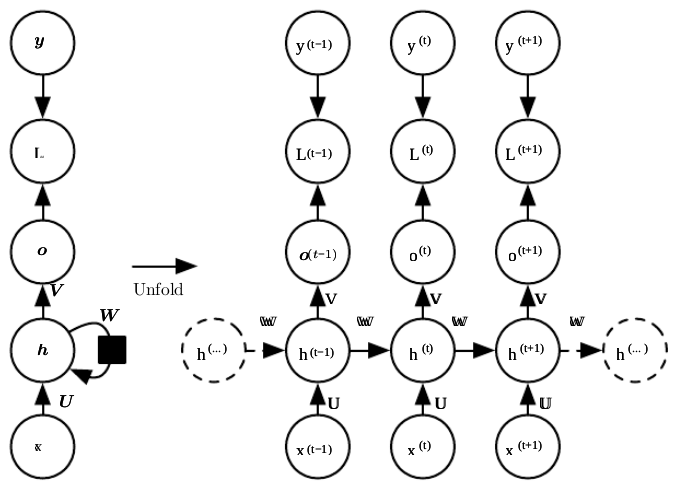
\includegraphics[scale=0.5]{img/grafo 2.png}
                \caption{Un grafo computacional que representa una RNN que produce una salida en cada paso de tiempo y tiene conexiones recurrentes entre las unidades ocultas. (Izquierda) la RNN y su pérdida dibujadas por conexiones recurrentes. (Derecha) Lo mismo pero visto como un grafo computacional desplegado donde cada nodo está asociado a un determinado paso de tiempo. }
                \label{grafo:rnn2}
            \end{figure}
            
        Desarrollamos las ecuaciones de la propagación hacia adelante para la RNN de la figura \ref{grafo:rnn2}. Como no se especifica la función de activación para las unidades ocultas vamos a suponer la tangente hiperbólica. Tampoco se especifica la forma exacta de la función de salida y pérdida, por lo que supondremos que la salida es discreta. Una forma natural para representar variables discretas es considerar la salida $o$ como si dieras las probabilidades logarítmicas sin normalizar de cada valor posible de la variable discreta. A continuación, podemos aplicar la operación softmax para obtener un vector $\hat{y}$ de probabilidades normalizadas sobre la salida. La propagación hacia adelante comienza en el estado inicial $h^{(0)}$. Luego para $t=1,...,\tau$ aplicamos las siguientes ecuaciones: 
        
            \begin{align}
                a^{(t)} &= b + Wh^{(t-1)} + Ux^{(t)},\\
                h^{(t)} &= \tanh{(a^{(t)})}, \\
                o^{(t)} &= c + Vh^{(t)}, \\
                \hat{y}^{(t)} &= softmax(o^{(t)})
            \end{align}
                

        \noindent donde los parámetros son los vectores de sesgo $b$ y $c$ junto con las matrices de pesos $U, V$ y $W$ para las conexiones de entrada a una unidad oculta, de una unidad oculta a uno de salida y de una unidad oculta otra oculta, respectivamente. Esto es un ejemplo de una red recurrente que asigna una secuencia de entrada a una secuencia de salida de la misma longitud. La pérdida total para una secuencia de valores $x$ y otra secuencia de valores $y$ sería sólo la suma de las pérdidas en todos los pasos de tiempo. Por ejemplo, si $L^{(t)}$ es la función de verosimilitud logarítmica negativa de $y^{(t)}$ dado $x^{(1)},...,x^{(t)}$, entonces
        
            \begin{align}
               L \big( \{x^{(1)},...,x^{(\tau)}\},\{y^{(1)},...,y^{(\tau)}\} \big) &= \sum_{t} L^{(t)}, \\
                &= -\sum_{t} \log p_{model} \big( y^{(t)} | \{x^{(1)},...,x^{(t)}\} \big)
            \end{align}  
        
        \noindent donde $p_{model} \big( y^{(t)} | \{x^{(1)},...,x^{(t)}\} \big)$ viene dado por la lectura de la entrada de $y^{(t)}$ del vector de salida del modelo  $\hat{y}^{(t)}$. El cálculo del gradiente de esta función de pérdida con respecto a los parámetros es una operación costosa ya que implica moverse de izquierda a derecha a través del grafo seguida de la propagación para atrás que va de derecha a izquierda. Tampoco se puede paralelizar (en el caso que estamos tratando, en otras RNNs, si se puede) ya que se realiza de manera secuencial por necesitar cada estado información del anterior. Tanto el tiempo de ejecución como el coste en memoria son $O(\tau)$. El algoritmo de backpropagation que se aplica en este tipo de redes neuronales se conoce como \textit{back-propagation a través del tiempo} (BBTT)\\ 
        
        \begin{figure}[htpb]
            \centering
            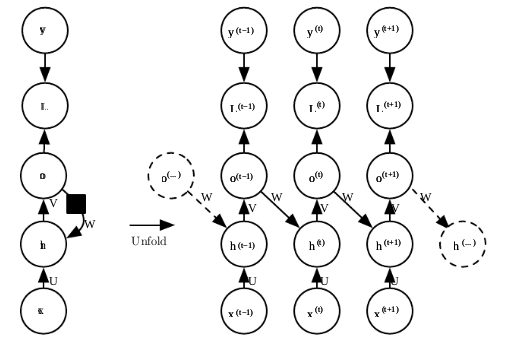
\includegraphics[scale=0.5]{img/rnn tipo.png}
            \caption{RNN cuya única recurrencia es la conexión de retroalimentación desde la salida a la capa oculta}
            \label{fig:rnn2tipo}
        \end{figure}
        
        
        
        \begin{figure}[htpb]
            \centering
            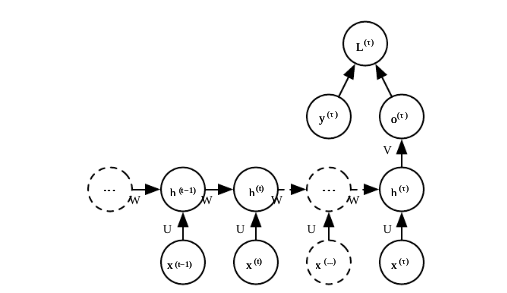
\includegraphics[scale=0.5]{img/rnn tercer tipo.png}
            \caption{Grafo desplecado de una RNN con una única salida al final de la secuencia. Esta red se suele usar para resumir una secuencia y producir una representación de tamaño fijo utilizada como entrada para el procesamiento posterior}
            \label{fig:rnn3tipo}
        \end{figure}
        
        
        
\section{Redes Neuronales Recursivas}

    Las redes neuronales recursivas representan una generalización de las redes recurrentes, con un tipo diferente de gráfico computacional que se estructura como un árbol profundo en lugar de la estructura de cadena de las RNNs. Un ejemplo típico es el de la figura \ref{fig:reNN}. Estas redes se introdujeron por primera vez en torno a 1990 y se suelen aplicar debido a su éxito en procesamiento de lenguaje natura y visión por computador entre otras disciplinas. Una cuestión que hay que pensar al usar estas redes es como estructurar el árbol. \\
        
    Una clara ventaja de estas redes sobre las recurrentes es que para una secuencia de la misma longitud $\tau$, la profundidad medida como el número de composiciones de operaciones no lineales puede ser drásticamente reducida de $\tau$ a $O(\log \tau)$, lo que ayuda a tratar las dependencias a largo plazo. \\
        
    Una cuestión abierta hoy en día es como estructurar de la mejor manera el árbol. Una propuesta es que se estructure de tal manera que no dependa de los datos, como un árbol binario equilibrado. Aunque la respuesta a esta cuestión puede ser tratada de diferentes maneras dependiendo del problema.
        
        \begin{figure}[htpb]
                \centering
                \includegraphics[scale=0.5]{recursivenn.png}
                \caption{La figura muestra un caso de aprendizaje supervisado en el que se proprociona un objetivo y se asocia a toda la secuencia. Una red recursiva tiene un grafo computacional que generaliza el de la red recurrente de una cadena a un árbol. Una secuencia de longitud variable $x^{(1)},...,x^{(t)}$ puede ser mapeada a una representación de tamaño fijo (la salida $o$) con un conjunto fijo de parámetros (matrices U, V y W) }
                \label{fig:reNN}
        \end{figure}
        
        
\section{El problema de la dependencias a largo plazo}\label{seccion:sorpresa}

    Una de las principales características de las redes neuronales recurrentes es que pueden conecta la información anterior con la actual, por lo que no resulta descabellado pensar que pueden recordar aspectos del pasado. Sin embargo, ¿Esto es así del todo?\\
    
    A veces, solo necesitamos mirar la información reciente para realizar la tarea actual como el ejemplo que se expuso al principio del capítulo sobre el \textit{Kilimanjaro}. En estos casos en los que la distancia entre la información relevante y el lugar en el que debe ser usada sea reducida, las RNNs pueden usar correctamente la información anterior que tienen. \\
    
    El otro extremo son los casos en los que necesitemos más contexto, es decir, cuando la distancia entre la información relevante y el lugar en el que debe ser usada es bastante amplia. Supongamos un texto en el que al principio del mismo empiece con \textit{Me crié en Italia} y tras todo un párrafo al final aparezca \textit{hablo fluidamente el italiano}. Si nuestro objetivo es predecir la última palabra del párrafo, \textit{italiano}, necesitamos usar la información del principio y es posible que la brecha entre la información relevante y el punto en que se necesita sea demasiado grande. \\
    
    Desgraciadamente, a medida que esa brecha crece, las RNN se vuelven incapaces de aprender a conectar la información. En teoría las RNN son absolutamente capaces de manejar estas dependencias a largo plazo. Pero en la práctica no es del todo así. Este problema fue estudiado por \textit{Hochreiter (1991)} y Bengio, et al. (1994) \cite{schmidhuber1997long, pascanu2013difficulty} y encontraron algunas razones fundamentales por las que podría ser difícil. No vamos a entrar en detalle ni a explicarlo de manera rigurosa pero sí que vamos a comentar por encima la causa del problema. \\

\subsection{Causa: Desvanecimiento/Explosión del gradiente}


        Las redes neuronales, en particular las RNNs, con grafos computacionales muy profundos presentan una dificultad a la que se debe enfrentar el algoritmo de optimización. Al aplicarse la misma operación de manera repetida en cada paso de tiempo provoca lo que se conoce como desvanecimiento y explosión del gradiente. \\
        
        Vamos a explicarlo primero con un ejemplo y posteriormente extendemos la explicación al caso de las RNN. Supongamos que un grafo computacional tiene un camino que consiste en multiplicar repetidamente por una matriz de pesos $W$. Después de $t$ unidades de tiempo, sería equivalente a multiplicar por $W^t$. Supongamos que $W$ tiene una descomposición en valores propios de la forma $W=V\cdot diag(\lambda) \cdot V^{-1}$, por lo que 
        
        \begin{equation}
            W^t = (V\cdot diag(\lambda) \cdot V^{-1})^t = V\cdot diag(\lambda)^t \cdot V^{-1} 
        \end{equation}
        
        Entonces, cualquier valor propio $\lambda_i$ que no esté en valor absoluto cerca de $1$ puede explotar si es bastante mas grande que $1$ o puede desvanecerse si está próximo a $0$. El problema de los gradientes evanescentes o explosivos se refiere al hecho de que los gradientes de un gráfico de este tipo también se escalan según $diag(\lambda_i)$. Por una parte, los gradientes evanescentes hacen que sea dificil saber en qué dirección deben moverse los pesos para mejorar la función de coste. Por otra parte, los gradientes explosivos hacen que el aprendizaje sea inestable. Es más común que ocurra el desvanecimiento que la explosión\\
        
        El principal problema es que los gradientes propagados a lo largo de muchas etapas tienden a desaparecer o a explotar. Si asumimos que los parámetros son tales que la RNN es estable (no explotan) la dificultad con las dependencias a largo plazo surge de los pesos exponencialmente más pequeños dados por las interacciones a largo plazo (que implican la multiplicación de muchos jacobianos) en comparación con las de corto plazo.\\
        
        Las RNNs traen consigo la composición de la misma función varias veces, una vez por unidad de tiempo. Estas composiciones pueden llegar a originar un comportamiento exageradamente no lineal. Esta composición de funciones se asemeja un poco a la multiplicación de matrices. Podemos pensar en la relación de recurrencia 
        
        \begin{equation}
            h^{(t)} = W^T \cdot h^{(t-1)}
        \end{equation}
        
        \noindent como una RNN muy simple que carece de una función de activación no lineal y de entradas. La relación anterior se puede ver también de la forma 
        
        \begin{equation}
            h^{(t)} = (W^t)^T \cdot h^{(0)}
        \end{equation}
        
        \noindent por lo que si $W$ admitiera una descomposición en valores singulares de la forma 
        
        \begin{equation}
            W = Q \Lambda Q^T
        \end{equation}
        
        \noindent siendo $Q$ una matriz ortogonal, se tendría que 
        
        \begin{equation}
            h^{(t)} = Q^T \cdot \Lambda^t \cdot Q \cdot h^{(0)}
        \end{equation}
        
        \noindent Por lo que tendríamos una situación igual a la del primer ejemplo. Los valores propios están elevados a la potencia de $t$, causando una explosión si son bastante más grandes que uno y un desvanecimiento si están próximos cero. Este problema es particular de las RNNs. 


\section{Long short-term Memory y GRU}

    Tras entender el concepto de RNNs ahora presentamos aquellas que vamos a emplear en la prácticas, las cuales reciben el nombre de LSTM (\textit{long short-term memory)} y GRU (\textit{Gated Recurrent unit}) las cuales se presentaron como solución al problema de la explosión y desvanecimiento del gradiente. \\

    \subsection{LSTM}

    Las LSTM (\textit{long short-term memory)} son un tipo especial de RNN, capaces de aprender dependencias a largo plazo. Fueron presentadas por \textit{Hochreiter y Schimidhuber} (1997) \cite{hochreiter1997long} y refinadas posteriormente por la comunidad investigadora. Hoy en día son muy usadas en multitud de campos, el más destacado es el proceseamiento del lenguaje natural. \\
    
    Este tipo de RNN está especialmente diseñada para evitar la dependencia a largo plazo, por lo que recordar información durante largos períodos de tiempo es su especialidad. Se basan en la idea de crear caminos a través del tiempo entre las entradas, salidas y estados internos que permitan recordar información u olvidarla si ya no es útil. De este modo se consigue que tengan derivadas que no se desvanezcan ni exploten. El objetivo es permitir a la red que acumule información como por ejemplo, la evidencia de una característica o categoría particular durante un largo periodo de tiempo y una vez que dicha información guardada se haya usado se permita que pueda ser olvidada. El hecho de olvidar la información no ocurre por arte de magia, sino que la red debe de ser capaz de aprender cuándo hacerlo y cuándo no.  \\
        
    Todas las redes neuronales recurrentes tienen la forma de una cadena en la que se repiten módulos, en las RNNs  típicas, estos módulos constan de una estructura muy simple formada por una operación no lineal elemento a elemento de una transformación afín de la entrada y las unidades recurrentes (Fig. \ref{fig:celda RNN}). En cambio, las LSTM, aunque presenten también una cadena de celdas repetidas, estas celdas cuentan con una recurrencia interna (bucle interno) además de la recurrencia externa de la RNN y una estructura mucho más sofisticada con puertas de control que manejan el flujo de la información. Los bucles internos producen trayectorias en las que el gradiente puede fluir durante largos periodos de tiempo. Un aspecto clave es que el peso de estos bucles esté condicionado por el contexto en vez de ser fijo, haciendo que el peso del bucle propio esté controlado por una unidad oculta (Fig. \ref{fig:celda LSTM}).\\
    
    
    \begin{figure}[H]
        \centering
        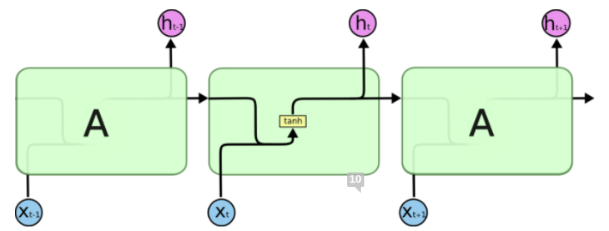
\includegraphics[scale=0.5]{rnng.png}
        \caption{Celda de una RNN común}
        \label{fig:celda RNN}
    \end{figure}
    
    \begin{figure}[H]
        \centering
        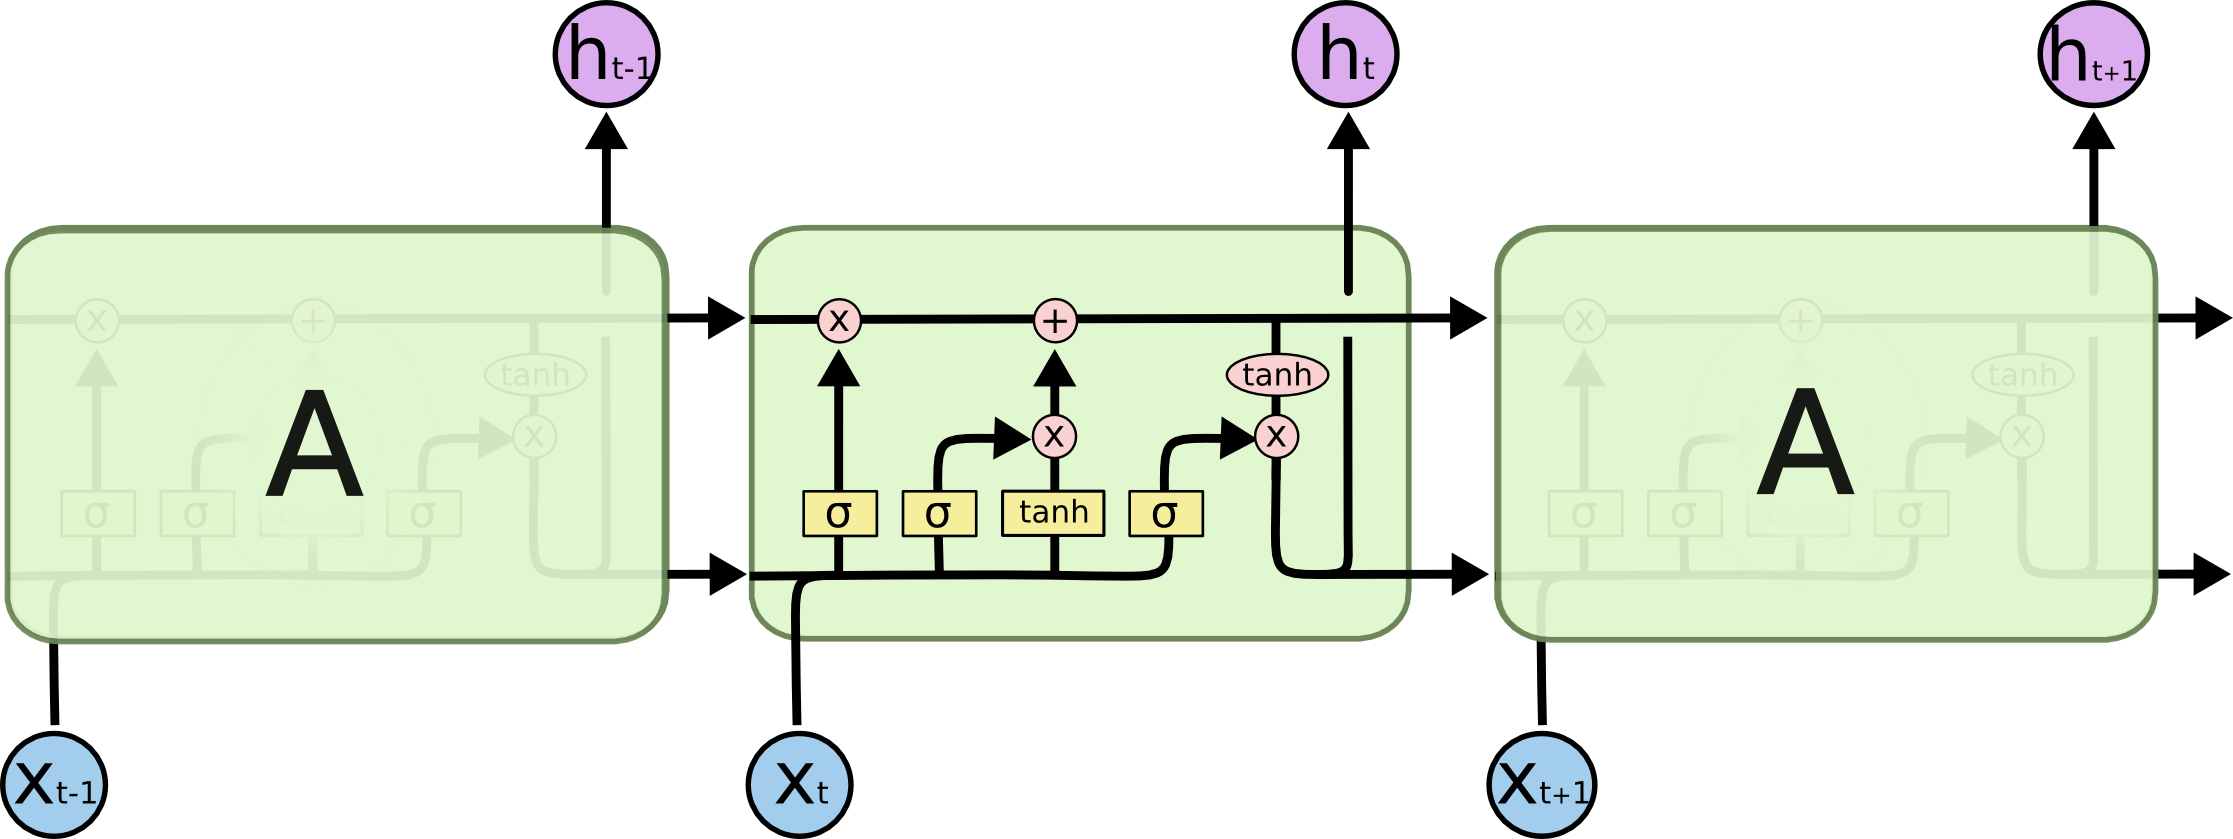
\includegraphics[scale=0.5]{lstmg.png}
        \caption{Celda de una LSTM. Podemos apreciar las dos recurrencias (interna y externa) y las puertas de control dentro de la celda}
        \label{fig:celda LSTM}
    \end{figure}
    
    De aquí en adelante usaremos diagramas para detallar el funcionamiento de una LSTM, por lo que usaremos la siguiente notación (Fig. \ref{fig:LSTM legend}) \\
    
    \begin{figure}[H]
        \centering
        \includegraphics[scale=0.7]{img/diagram legend.png}
        \caption{Notación para los diagramas.}
        \label{fig:LSTM legend}
    \end{figure}
    
    La clave de las LSTMs es el estado de la celda, que en un tiemop $(t)$ y una celda $i$, se representa por $C_i^{(t)}$ y viene dada por la línea horizontal que atraviesa la parte superior del diagrama \ref{fig:LSTM estado} y resaltada en negro. El estado de la celda consta de un bucle interno y es una especie de cinta transportadora. Corre en línea recta por toda la cadena con solo algunas transformaciones lineales menores. Es muy fácil que la información fluya a lo largo de ella sin cambios. \\
    
    	 \begin{figure}[H]
	        \centering
	        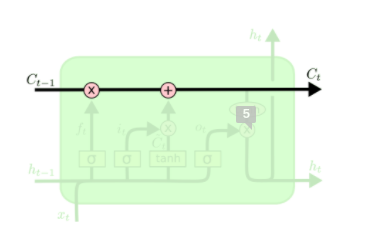
\includegraphics[scale=0.7]{d1.png}
	        \caption{Estado de una celda LSTM}
	        \label{fig:LSTM estado}
	    \end{figure}
	    
	 Como ya se comentó, las LSTMs tienen la habilidad de eliminar o añadir información al estado de la celda gracias a las puertas. Estas están compuestas por una función sigmoidal y una operación de multiplicación punto a punto. La función sigmoidal (Fig. \ref{fig:LSTM sigmoidal}), cuya salida está comprendida entre cero y uno viene a indicar cuánta información deja pasar. Un valor de cero significa que no deja nada pasar mientras que un valor de uno significa que lo deja todo. Una celda LSTM tiene tres puertas de este tipo para proteger y controlar el estado de la celda. \\ 
	 
	 \begin{figure}[H]
	     \centering
	     \includegraphics[scale=0.8]{img/LSTM sigmoidal.png}
	     \caption{Capa Sigmoidal. Esta capa controla la cantidad de información que se deja pasar.}
	     \label{fig:LSTM sigmoidal}
	 \end{figure}
	    
	     
	 El primer paso es decidir que información vamos olvidar del estado de la celda empleando para ello la puerta de olvido (Fig. \ref{fig:dd2}). Los pesos del bucle interno son controlados por esta puerta que recibe como entrada los vectores $x^{(t)}$ y $h^{(t-1)}$ que contienen los inputs de entrada y la información de las celdas anteriores. Devuelve un vector conteniendo números entre $0$ y $1$ al estado $C_{t-1}$ para decidir qué olvidar, qué no olvidar y cúanto olvidar. \\
	    
	    
	    \begin{figure}[H]
	      \centering
	      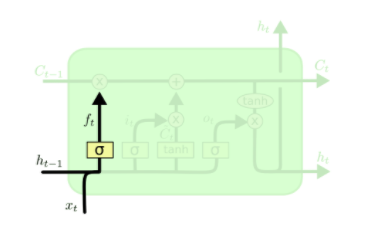
\includegraphics[scale=0.7]{dd2.png}
	      \caption{Puerta de olvido}
	      \label{fig:dd2}
	    \end{figure}
	    
	 La puerta de olvido para un instante de tiempo $(t)$ y una celda $i$ la vamos a modelar por la función $f_i^{(t)}$ cuya expresión viene dada por
	 
	 \begin{equation}\label{eq:lstm_f}
	     f^{(t)}_i = \sigma \Big( b^f_i + \sum_j U_{i,j}^f x^{(t)}_j + \sum_j W_{i,j}^f h^{(t-1)}_j \Big)
	 \end{equation}
	    
	\noindent donde $b_i^f, U_i^f$ y $W_i^f$ son respectivamente el sesgo, los pesos de entrada y los pesos recurrentes para la puerta de olvido en la celda $i$. A modo de ejemplo, imaginemos que tenemos un modelo de un lenguage el cual intenta predecir la siguiente palabras basándose en las anteriores. En este problema la celda de estado puede tener codificado el género del sujeto o la persona, entonces un cambio del mismo supondría la necesidad de eliminar la información del sujeto anterior anterior así como por ejemplo, determinantes, conjugaciones verbales o pronombres. Es en este punto donde decidimos olvidar toda esa información. \\
	  
    El siguiente paso es decidir qué información vamos a almacenar en el estado de la celda, esto se hace en dos fases. La primera es decidir qué valores se van a actualizar usando una función sigmoidal conocida como la \textit{puerta de entrada} (Fig. \ref{fig:LSTM input gate}), $g_i^{(t)}$. Después, una capa $\tilde{C}_t$, con una función $tanh$ (también puede ser una función sigmoidal) crea un vector con posibles candidatos a ser añadidos. En el ejemplo, es en este punto donde nos gustaría añadir el género del nuevo sujeto al estado de la celda para reemplazar el antiguo que estamos olvidando. Las expresiones vienen dadas por
    
    \begin{equation}
    \begin{aligned}
        g^{(t)}_i & = \sigma \Big( b^g_i + \sum_j U_{i,j}^g x^{(t)}_j + \sum_j W_{i,j}^g h^{(t-1)}_j \Big) \\
        \tilde{C}^{(t)} & = \tanh \Big( b^C_i + \sum_j U^C_{i,j}x^{(t)}_j + \sum_j W^C_{i,j} h^{(t-1)}_j \Big)
    \end{aligned}
    \end{equation}
    
    
    \noindent donde $b^g, b^C, U^g, U^C, W^g, W^C$ son los sesgos, los pesos de entrada y los pesos recurrentes asociados a la puerta de entrada y la función que establece los candidatos respectivamente. \\
	    
    

	    \begin{figure}[H]
	      \centering
	      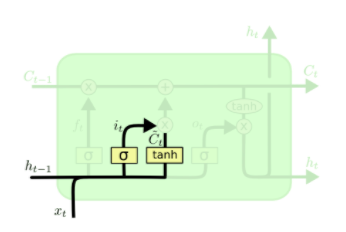
\includegraphics[scale=0.7]{dd3.png}
	      \caption{Puerta de entrada. En este diagrama la función $g^{(t)}$ viene representada por }
	      \label{fig:LSTM input gate}
	    \end{figure}
	  
	 \noindent En la segunda fase se combinan la salida de la puerta de entrada y este nuevo vector de candidatos para actualizar el estado antiguo al estado nuevo (Fig. \ref{fig:LSTM update}). Los pasos anteriores ya decidieron que información usar para ello, por tanto solo queda multiplicar el antiguo estado por la salida de la puerta de olvido y sumarlo a la multiplicación de la salida de la puerta de entrada con el vector de candidatos creado por la función $\tilde{C}^{(t)}$. Para el ejemplo del modelo de lenguaje, aquí es donde dejaríamos la información sobre el género del sujeto anterior y añadiríamos la nueva información. 
	 
	 
	   \begin{figure}[H]
	      \centering
	      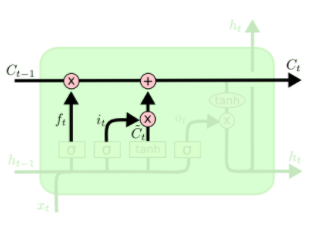
\includegraphics[scale=0.5]{dd5.png}
	      \caption{Actualización}
	      \label{fig:LSTM update}
	   \end{figure}	  

    \begin{equation}
	     C^{(t)}_i = f^{(t)}_i * C^{(t-1)}_i + g^{(t)}_i * \tilde{C}_i^{(t)}
	 \end{equation}

    Por último, se decide qué o cuánta información va a ser sacada como salida de la capa oculta, la cual se representa por $h_i^{(t)}$ y se le conoce puerta de salida (Fig. \ref{fig:LSTM output gate}). Primero se aplica una función sigmoidal que decide qué partes del estado van a ser usadas para la salida. Tras ello, se aplica una función $tanh$ (que mapea los valores entre $-1$ y $1$) al estado actual y se multiplica por la salida de la sigmoidal. 
    
    \begin{equation}
    \begin{aligned}
        o^{(t)}_i & = \sigma \Big( b^o_i + \sum_j U^o_{i,j} x^{(t)}_j + \sum_j W^o_{i,j} h^{(t-1)}_j \Big) \\
        h^{(t)}_i & = tanh \big( C^{(t)}_i \big) * o^{(t)}_i
    \end{aligned}
    \end{equation}

    \noindent donde los parámetros $b^o, W^o$ y $U^o$ son los sesgos, los pesos de entrada y los pesos recursivos respectivamente. En el ejemplo del modelo de lenguaje, si nos topamos con un nuevo sujeto, podríamos querer emitir información relevante para el verbo, como por ejemplo, decir si el sujeto está en singular o plural para obtener información sobre la conjugación del verbo. 

	   \begin{figure}[H]
	      \centering
	      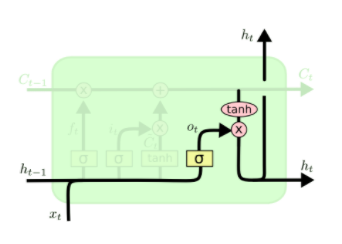
\includegraphics[scale=0.5]{dd6.png}
	      \caption{Puerta de salida}
	      \label{fig:LSTM output gate}
	   \end{figure}
    

    \subsubsection{Variantes}
    

    El ejemplo anterior es de una arquitectura en concreto, de hecho, la mayoría de LSTMs usadas son variaciones de esta última. Por ejemplo, en la imágenes \ref{fig:lstm_v1} y \ref{fig:lstm_v2} tenemos dos variantes. 
	   
	   \begin{figure}[H]
	       \centering
	       \includegraphics[scale=0.5]{dd7.png}
	       \caption{Variación 1: Se introducen \textit{peephole connections} permitiendo que las puertas de olvido y salida puedan consultar el estado. Hay otras muchas variantes de este modelo en función de que puertas tengan las \textit{peephole connections.}}
	       \label{fig:lstm_v1}
	   \end{figure}
	   
	   
	   \begin{figure}[H]
	       \centering
	       \includegraphics[scale=0.5]{dd8.png}
	       \caption{Variación 2: En esta arquitectura en vez de decidir de manera separada que información vamos a olvidar y a añadir, se toma la decisión de forma conjunta.}
	       \label{fig:lstm_v2}
	   \end{figure}
	    
	    
    \subsection{GRU}
    
        Las GRU (Fig. \ref{fig:gru}) \cite{chung2014empirical} son otro tipo de redes neuronales recurrentes, o incluso también pueden ser vistas como una variante de las LSTM cuya principal diferencia radica en que éstas usan una puerta que controla simultáneamente la parte que olvida y la parte que actualiza. Al igual que las LSTMs, las GRUs cuentan con una gran cantidad de variaciones. Su expresión viene por  \\
        
        \begin{equation}
            h^{(t)} = u^{(t-1)}_i h^{(t-1)}_i + ( 1 - u^{(t-1)}_i) \sigma \Big( b_i + \sum_j U_{i,j} x^{(t)}_j + \sum_j W_{i,j} r^{(t-1)}_j h^{(t-1)}_j \Big),
        \end{equation}
        
        \noindent donde $u$ representa la puerta de actualización y $r$ la de reinicio y cuyas ecuaciones son, 
        
        \begin{equation}
            u^{(t)}_i = \sigma \Big( b^u_i + \sum_j U^n_{i,j} x^{(t)}_j + \sum_j W^u_{i,j}h^{(t)}_j\Big)
        \end{equation}
	    
	    \begin{equation}
	        r^{(t)}_i = \sigma \Big( b^r_i +  \sum_j U^r_{i,j} x^{(t)} + \sum_j W^u_{i,j}h^{(t)}_j \Big)
	    \end{equation}
	    
	    
	    \begin{figure}[H]
	      \centering
	      \includegraphics[scale=0.6]{dd9.png}
	      \caption{Ejemplo de un arquitectura de GRU. En este ejemplo podemos ver apreciar como se juntan la puerta de olvido y actualización en una. También se aprecia la fusión del estado de la celda con el estado de la unidad oculta. Este modelo se está convirtiendo cada vez más popular.}
	      \label{fig:gru}
	    \end{figure}
	    
	   

    


\endinput